\documentclass[conference]{IEEEtran}
\usepackage[spanish]{babel}
\usepackage{blindtext, graphicx}
\usepackage{mdwmath}
\usepackage{mdwtab}

\begin{document}
\title{ Histograma de una imagen en escala de grises}
\author{\IEEEauthorblockN{Walter Alejandro Moreno Ram\'irez}
\IEEEauthorblockA{Departamento de Estudios Multidisciplinarios\\
Universidad de Guanajuato\\
Yuriria, Guanajuato\\
Correo: wa.morenoramirez@ugto.mx}}

\maketitle
\renewcommand\abstractname{Abstract}
\begin{abstract}
This article describes a histogram, what is the importance of a histogram in the analysis of images and how to make a histogram, besides adding examples of images with their respective histograms. \\
\end{abstract}

\begin{IEEEkeywords}
Pixel, histograma, brillo, contraste, funci\'on, c++, OpenCV.
\end{IEEEkeywords}

\IEEEpeerreviewmaketitle
\section{Introducci\'on}
El histograma de una imagen digital es una estimaci\'on de la ocurrencia o la frecuencia con la que un valor en escala de grises se repitem, Se representa por la Ecuaci\'on (1).\\
\begin{equation}
h(r_k) = n_k
\end{equation}
Donde $r_k$ es el k-esimo elemento de la escala de grises y $n_k$ es el n\'umero de pixeles que tiene la imagen con el nivel de gris $r_k$.\\
Es muy com\'un que se normalice el histograma, esto se logra diviendo cada elemento del histograma entre el n\'umero total de elemento o p\'ixeles de la im\'agen y est\'a dado por la Ecuaci\'on (2).
\begin{equation}
p(r_k) = \frac{n_k}{n}
\end{equation}
para $k = 0,1,....,L-1$ \\\\
Un aspecto a resaltar es que la suma de todos los componentes de un histograma normalizado es igual a 1.\\\\
El histograma se visualiza en una gr\'afica de barras, lo que nos muestra como es la distribuci\'on de la escala de grises en toda la imagen como se muestra en la Figura 1. Este grafico es muy utilizado en otras t\'ecnicas de procesamiento de im\'agenes, como lo son la compresi\'on y segmentaci\'on.
\begin{figure}[h]
	\begin{center}
		\setlength{\unitlength}{0.00105in}
		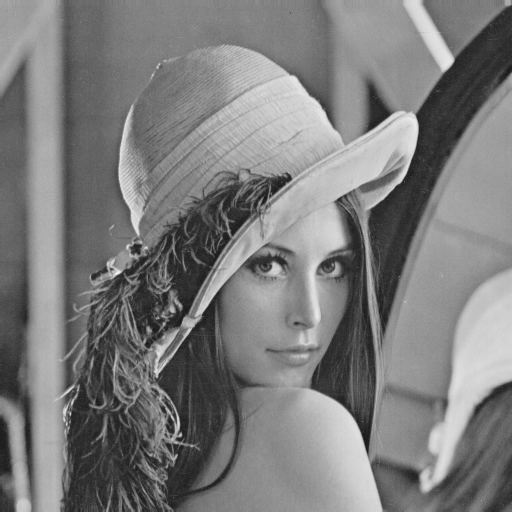
\includegraphics[scale=0.15]{./images/Imagen1.png}
		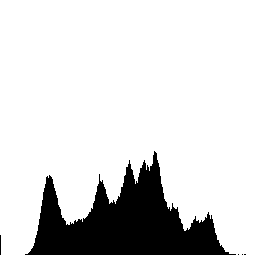
\includegraphics[scale=0.55]{./images/Grafica1.png}
	\end{center}
	\caption{\emph{Imagen y su histograma.}}
\end{figure}

\textbf{Secciones}
\begin{itemize}
    \item Metodolog\'ia
    \item Resultados
    \item Conclusiones
\end{itemize}

\section{Metodolog\'ia}
Para realizar esta pr\'actica fue necesario basarse en una pr\'actica anterior, donde se creo una imagen con un color y taman\~o definidos con un \'unico canal, adem\'as de abrir y manipularla una imagen. El c\'odigo fue programado en C++ con OpenCV.\\
Una vez teniendo esto se procede a obtener el histograma de la imagen, para ello se creo una funci\'on que como par\'ametros recibe la imagen y dentro obtiene el histograma de acuerdo al pseudocodigo de la Figura 2. Cabe resaltar que se utiliza una imagen con 3 canales de color, pero para obtener la ocurrencia de los datos s\'olo se considerar\'a el canal 0\'o el canal azul.\\

\begin{figure}[h]
	\begin{center}
		\setlength{\unitlength}{0.00105in}
		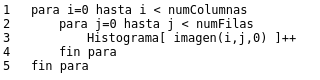
\includegraphics[scale=0.50]{./images/pseudocodigo1.png}
	\end{center}
	\caption{Pseudocodigo de un algoritmo para obtener el histograma de una imagen.}
\end{figure}

Donde numFilas y numColumnas representan, del taman\~no de la imagen, largo y ancho respectivamente. Dentro del vector Histograma se guarda la frecuencia con que ocurre un nivel de gris en la imagen, por esa raz\'on es que como \'indice se utiliza el valor que se obtiene de cada pixel, este valor ser\'a un valor entre 0 y 255 lo cual aumentar\'a en una unidad dentro del vector Histograma.\\\\
Una vez obtenido el histograma se procede a normalizarlo, de acuerdo a la Ecuaci\'on (2) para normalizar el histograma es necesario dividir cada uno de los elementos entre el total de elementos de la imagen, esta cantidad se obtiene del producto $largo*ancho$. \\\\
Para mostrar el histograma se cre\'o una funci\'on que como par\'ametros recibe un vector. Dentro de la funci\'on se crea imagen con los tres canales en 255 lo que resulta de una imagen con color blanco. Para dibujar el histograma en la imagen se sigue el pseudocodigo de la Figura 3.\\

\begin{figure}[h]
	\begin{center}
		\setlength{\unitlength}{0.00105in}
		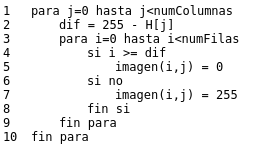
\includegraphics[scale=0.45]{./images/pseudocodigo21.png}
	\end{center}
	\caption{Pseudocodigo para dibujar un histograma en una imagen.}
\end{figure}

La asignaci\'on $dif = 255-H[j]$ indica una diferencia entre la altura m\'axima y el valor obtenido del histograma normalizado en el \'indice $j$, esto nos da como resultado la altura que tendr\'a la ocurrencia del nivel de gris $j$ en la gr\'afica.\\ Para poder dibujar dicha altura es necesario utilizar el segundo bucle, este se encargar\'a de recorrer todas las filas con el contador $i$ y hacer una comparaci\'on. Si $i >= dif$, si el contador $i$ es mayor o igual al valor obtenido en $dif$ entonces pondr\'a ese pixel en bajo, indicado por la l\'inea $imagen(i,j)=0$ de lo contrario el valor que no cumpla la condici\'on tendr\'a se pondr\'a ese pixel en alto, $imagen(i,j)=255$\\\\
Como etapa final se muestran la imagen y el histograma en una ventana individual.\\\\

\section{Resultados}
Se probaron 3 im\'agenes distintas con diferentes distribuciones de la escala de grises; oscuro, iluminado y balanceado.\\
La primer imagen muestra una tendencia al color negro, y pocos pero visibles valores que van desde el gris claro hasta el blanco. Esto se ve m\'as facilmente en la Figura 4 y la Figura 5.

\begin{figure}[h]
	\begin{center}
		\setlength{\unitlength}{0.00105in}
		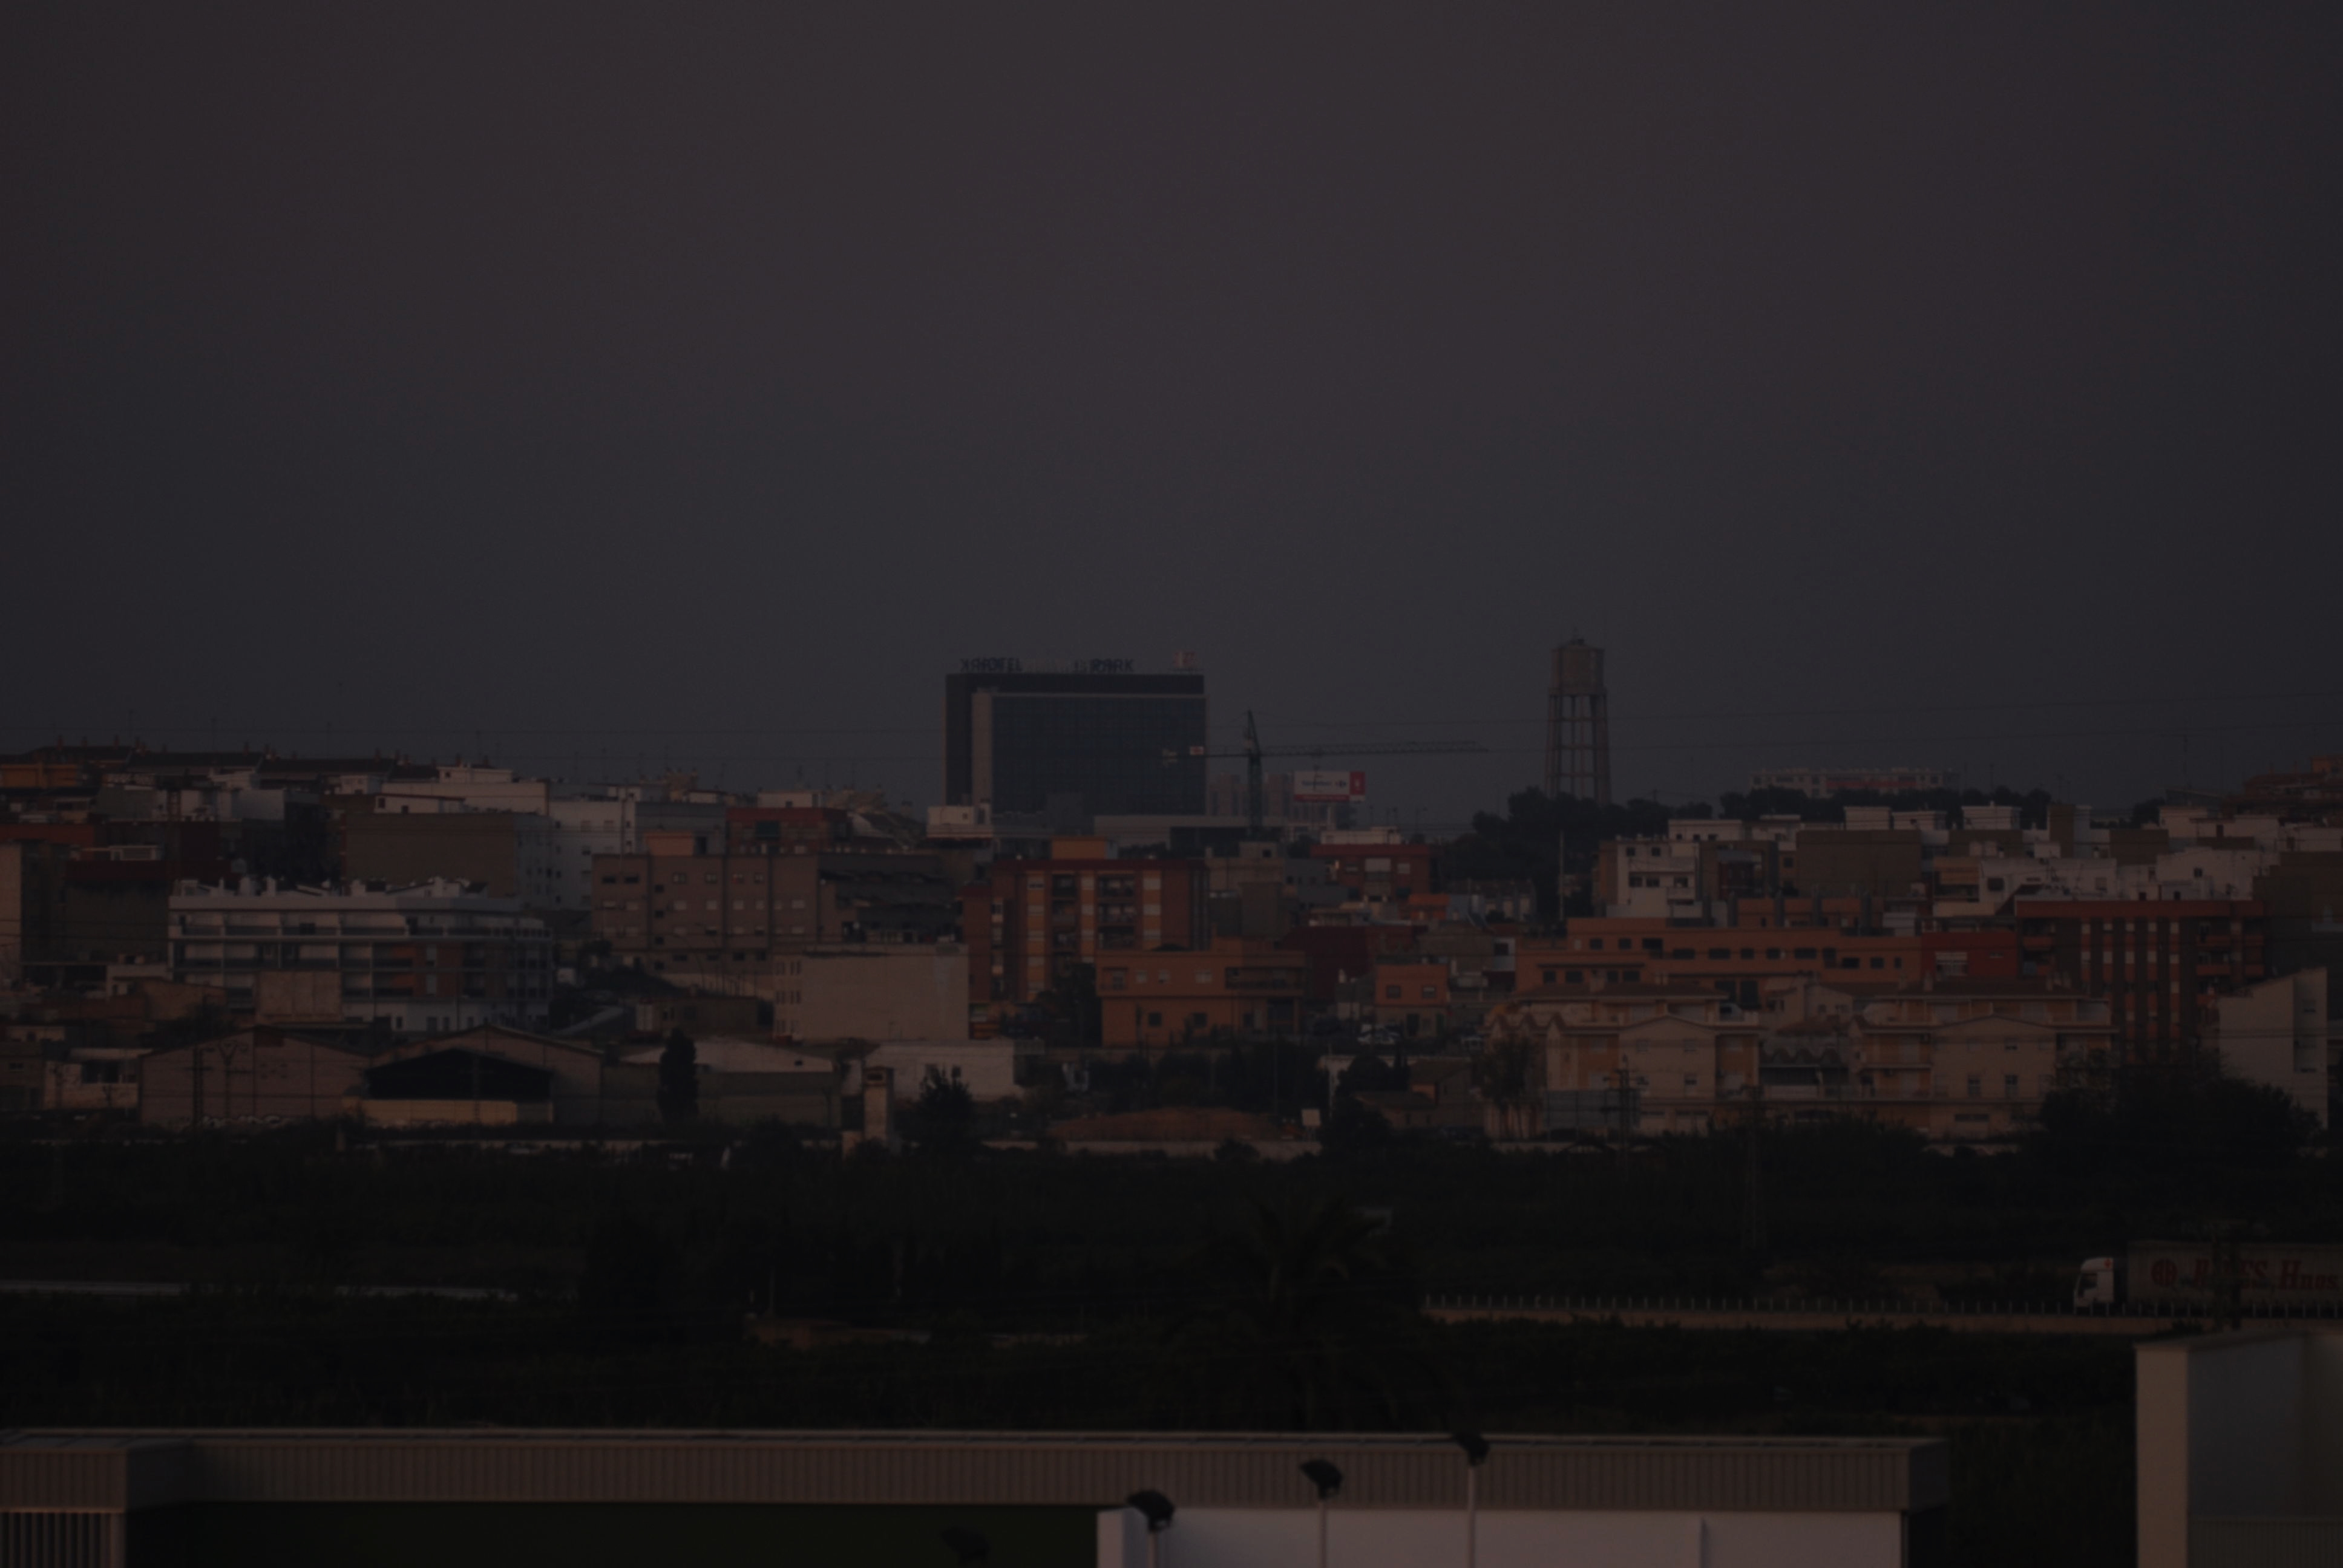
\includegraphics[scale=0.040]{./images/Iprueba1.jpg}
	\end{center}
	\caption{Primer imagen de prueba, bajo contraste.}
\end{figure}

\begin{figure}[h]
	\begin{center}
		\setlength{\unitlength}{0.00105in}
		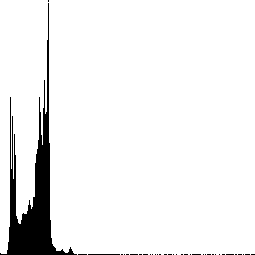
\includegraphics[scale=0.70]{./images/Hprueba1.png}
	\end{center}
	\caption{Histograma de la primer imagen de prueba con bajo contraste.}
\end{figure}

\newpage
La segunda imagen de prueba es una imagen que tiene niveles de gris intermedios, por lo tanto da como resultado una imagen balanceada en cuanto a tonalidades de grises, pero con un pico en el centro como se muestra en las Figuras 6 y el histograma de la Figura 7.\\

\begin{figure}[h]
	\begin{center}
		\setlength{\unitlength}{0.00105in}
		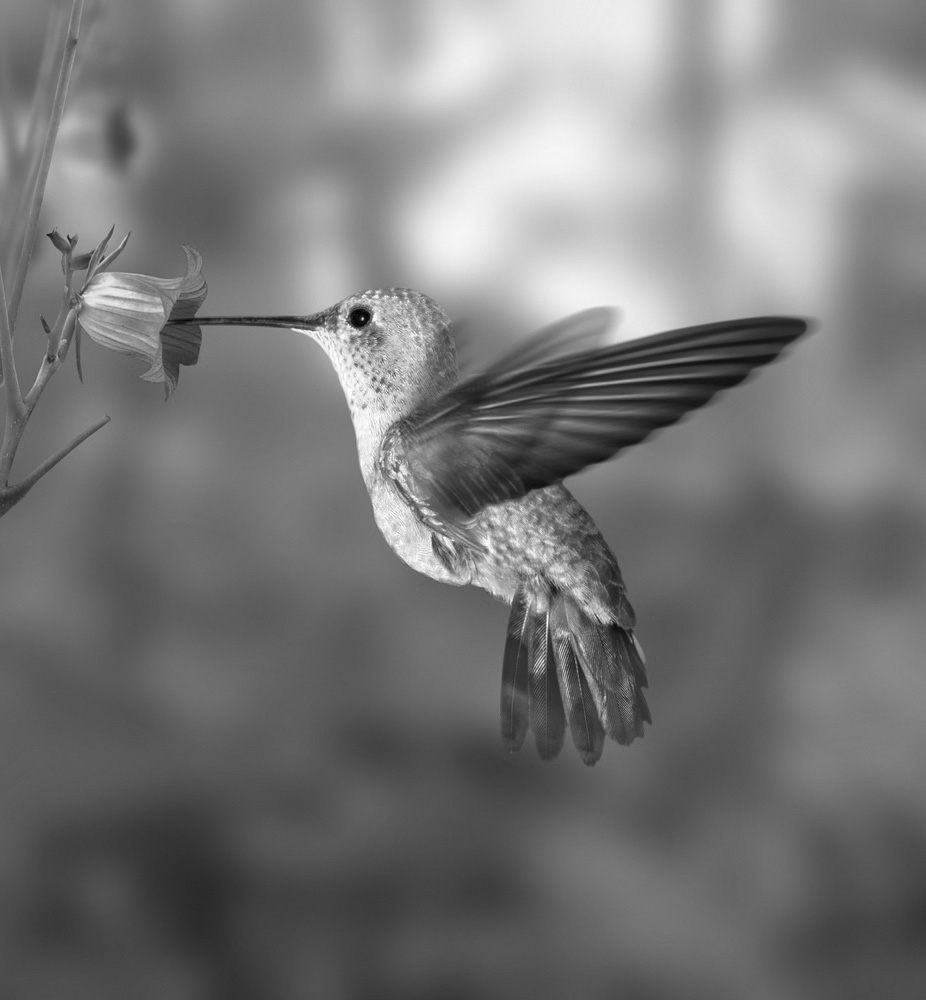
\includegraphics[scale=0.18]{./images/Imprueba2.jpg}
	\end{center}
	\caption{Primer imagen de prueba, niveles intermedios de grises.}
\end{figure}

\begin{figure}[h]
	\begin{center}
		\setlength{\unitlength}{0.00105in}
		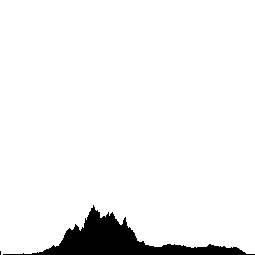
\includegraphics[scale=0.70]{./images/Hprueba2.png}
	\end{center}
	\caption{Histograma de la segunda imagen con niveles de grises intermedios.}
\end{figure}

La tercera imagen de prueba es una imagen que tiene un contaste alto, por lo tanto da como resultado una imagen donde se puede diferenciar dos tonos totalmente opuesto como lo es el blanco y el negro, lo cual se aprecia mejor por los picos en ambos extremos, tal como se muestra en las Figuras 8 y el histograma de la Figura 9.

\begin{figure}[h]
	\begin{center}
		\setlength{\unitlength}{0.00105in}
		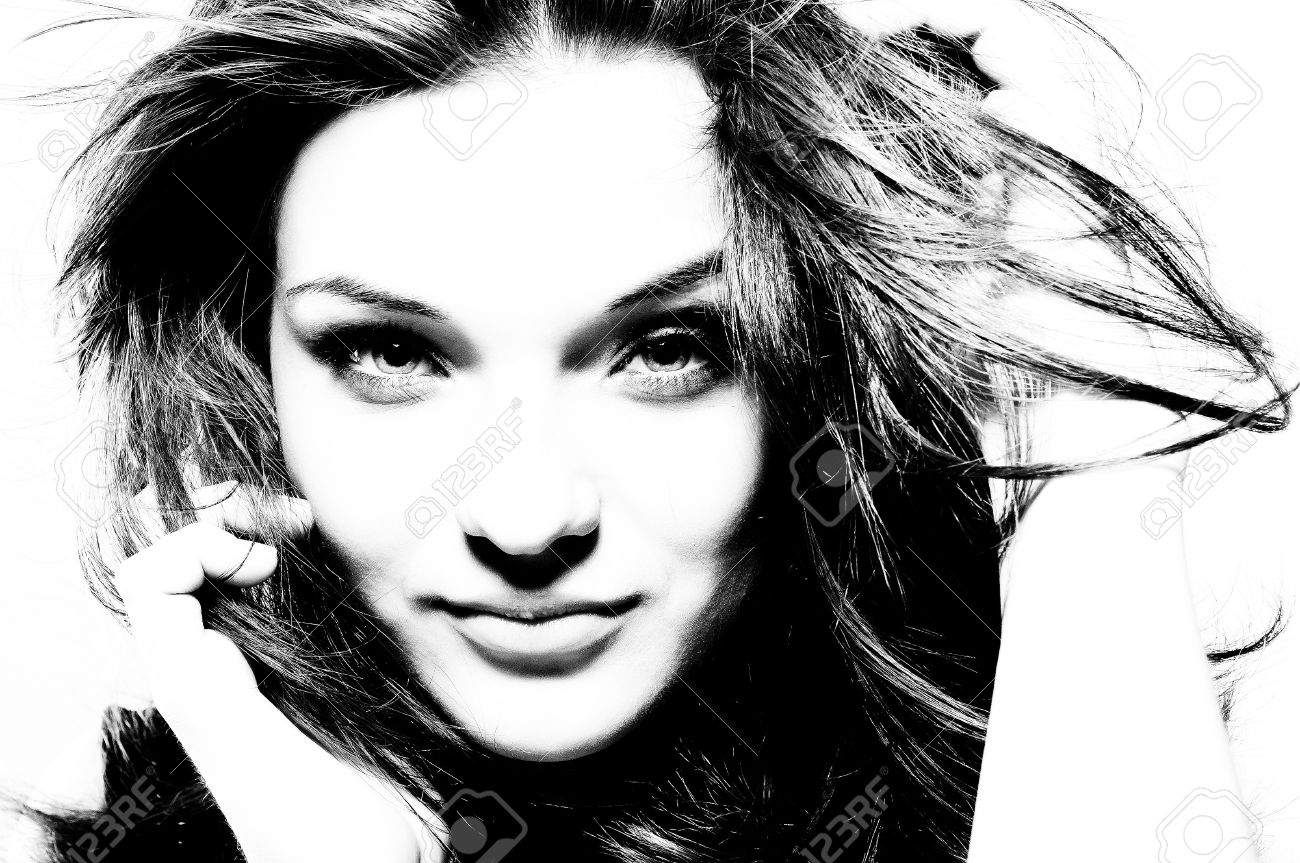
\includegraphics[scale=0.13]{./images/Imprueba3.jpg}
	\end{center}
	\caption{Primer imagen de prueba, contraste balanceado.}
\end{figure}

\begin{figure}[h]
	\begin{center}
		\setlength{\unitlength}{0.00105in}
		
\includegraphics[scale=0.70]{./images/Hprueba3.png}
	\end{center}
	\caption{Histograma de la segunda imagen de prueba con contraste balanceado.}
\end{figure}

\section{Concluciones}
A lo largo de la pr\'actica se aprendio la importancia del histograma para analizar una imagen, tener el conocimientos de las ocurrencias con que un nivel de gris est\'a presente en una imagen es de mucha ayuda. Obtener el histograma de una imagen puede servir para identificar figuras planas que est\'en llenas de un color uniforme, adem\'as de las aplicaciones que tiene para el procesamiento de im\'agenes.

%\begin{thebibliography}{1}
%    \bibitem{IEEEhowto:kopka}
%    H.~Kopka and P.~W. Daly, \emph{A Guide to \LaTeX}, 3rd~ed.\hskip 1em plus
%      0.5em minus 0.4em\relax Harlow, England: Addison-Wesley, 1999.
%\end{thebibliography}

%\begin{IEEEbiography}[{\includegraphics[width=1in,height=1.25in,clip,keepaspe%ctratio]{picture}}]{John Doe}
%\blindtext
%\end{IEEEbiography}

\end{document}